\chapter{引言}
\label{cha:intro}

\section{研究背景与意义}
合成孔径雷达(synthetic aperture radar,SAR)~\cite{Knight2018Synthetic}以微波遥感的形式进行对地观测,可以不受天气、光照等自然
条件的影响,具有全天候、全天时的实时对地观测能力。鉴于SAR系统可以提供丰富的地物散射特征等信息,目前其被广泛应用于
自然灾害评估,海洋维权,对地侦察,资源勘探等领域~\cite{Moreira2013A}。SAR技术自从20世纪50年代诞生以来,已经取得了
长足的发展。最初其被应用于侦察和检测人造目标等军用领域,进入到七十年代,一些用来探测地表物理特征的民用机载SAR系统被相继研发。
1978年,第一颗民用SAR卫星Seasat发射。二十世纪九十年代欧洲、日本、加拿大分别发射了ERS-1/2、JERS-1、Radarsar-1星载SAR系统。21世纪进入
SAR系统发展的黄金时代,如今在轨运行的星载SAR系统超过20个,我国于2016年发射了高分三号遥感卫星(GF-3),这是一颗C波段分辨率达
到1米的多极化合成孔径雷达卫星。

广泛的应用场景需求在不断推动着SAR成像技术的迅猛发展,起初SAR系统只能以一种收发电磁波的模式去获取数据,工作频段、角度单一。如今SAR系统成像模式日渐
多样化,产生了多极化,多角度,多波段,多识相的组合观测模式。相较于单极化SAR系统,多极化SAR可以采用多种组合观测模式去获得地物目标的完备的散射信息。
目前SAR成像技术在向高空间,时间分辨率的方向发展,对于高分辨SAR影像的后处理以满足各领域应用需求等前沿科学问题正在引发学者广泛关注~\cite{李德仁2012高分辨率对地观测的若干前沿科学问题}。

近几年,图形处理器(GPU)因其高效的计算性能引起了科研人员的广泛关注。最初图像处理器作为协处理器仅被用来加速图像处理与实时图像渲染以提供平滑与流畅的屏幕图形
显示。如今随着深度学习的快速发展,GPU因其强大的数据处理能力与高内存带宽已经成为神经网络训练的标配。在SAR领域,GPU也被广泛应用SAR图像的生成与后处理~\cite{Jin2012GPU,Liu2009An}。与此同时,GPU编程接口CUDA也一直与时俱进,其提供了一套基于C/C++的API
以便捷开发人员创建可以在其上运行的软件。

海上舰船目标检测与识别是极化SAR重要应用之一。我国海域辽阔,近些年来海上安全形势日趋严峻,海洋管控能力亟待提升。
基于极化SAR的舰船目标检测与识别对于航线管理,海上救援,航洋权益争端等具有非常重要的意义。然而传统的极化SAR目标识别方法
存在着计算复杂度高,耗时长等问题。针对此问题,我们基于CPU+GPU的异构架构将SAR目标检测算法中可并行的部分附加
到高速的GPU中去执行,从而全面提升SAR系统对目标快速识别与处理的能力。

  \begin{figure}[H] % use float package if you want it here
    \centering
    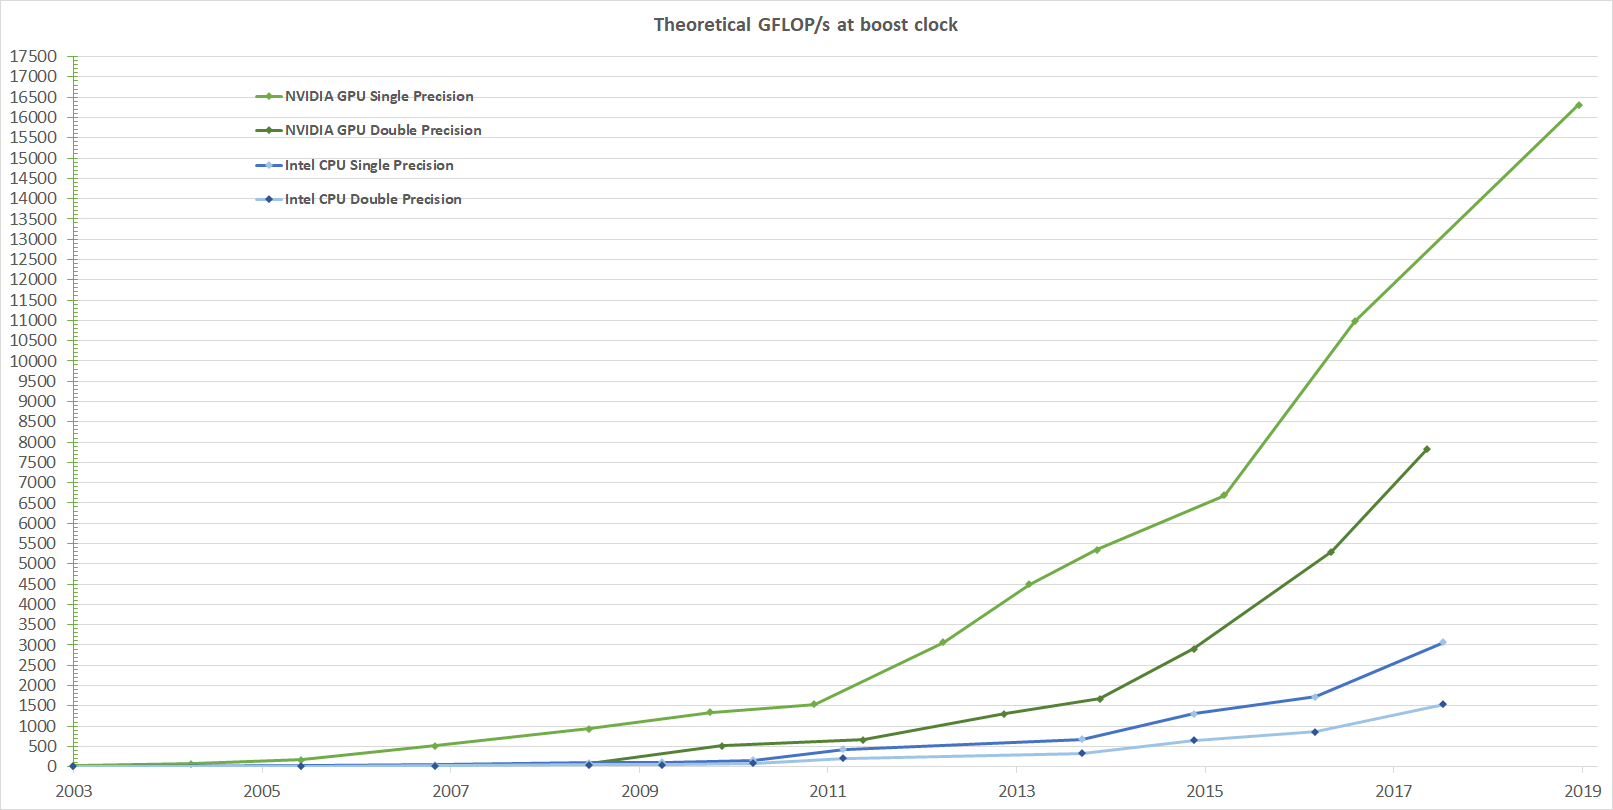
\includegraphics[width=0.8\textwidth]{GPUspeed.png}
    \caption{CPU和GPU浮点运算比较}
    \label{fig:chap1:GPUspeed}
  \end{figure}

\section{研究现状与进展}
  本节介绍SAR图像舰船检测方法研究与进展,包含了单极化SAR图像舰船检测与极化SAR图像舰船目标检测。
\subsection{单极化SAR舰船目标检测}
    通常星载SAR系统可以对大范围海面进行成像,对于原始单通道SAR图像数据,舰船目标检测主要包含了以下
    几个过程:海陆分割,截取含有潜在目标的候选检测区域,使用目标检测算法鉴别候选区域中的
    舰船像素与杂波像素~\cite{article}。目前大多数检测算法都是依据舰船目标与海面后的向散射特性的差异来进行
    鉴别。舰船目标包含大量二面角,后向散射系数较高,在强度图像中表现为一块高亮区域,而海杂波则为
    无规则的灰暗斑点噪声的形态。

    在基于幅值的单极化SAR图像舰船目标检测方法中,应用最广泛的为基于恒虚警率(CFAR)的舰船检测方法。CFAR检测方法根据滑动窗选择
    待检测像素周围的海杂波像素,然后按照事先提出的统计分布模型依据选择的海杂波像素去估计杂波分布参数,得到杂波分布
    后根据恒虚警率$P_{FA}$去计算自适应分割阈值$T$,当待检测像素值大于阈值$T$时将该像素判定为舰船像素~\cite{王兆成2017基于单极化}。
    对于恒虚警率舰船检测方法,其检测精度主要受到两个因素的影响,雷达系统本身的参数,如极化模式、入射角等,另一个是成像区域海况条件如风速
    风向等。

    对于海杂波的统计建模方法,Novak\cite{Novak}提出了双参数CFAR检测方法,该方法采用高斯分布对海杂波进行统计建模,实验结果
    表明在低分辨率匀质杂波的条件下,双参数CFAR检测器拥有较好的检测性能。此外研究人员还采用了其他分布模型如瑞利分布、K分布、对数正态分布
    、Weibull分布来描述海杂波分布特性,经实验验证,这些统计模型都可以有效区分SAR图像中的舰船目标与背景杂波~\cite{Carretero2010Statistical}。虽然有很多可供
    选择的统计分布模型,但是在高分辨率的复杂海洋场景中,这些模型对杂波的拟合精度依然不能满足检测要求,于是一些学者提出了非参数化的检测方法。Jiang et al.~\cite{Q2000Automatic}提出了
    概率神经网络(Probability neural newworks, PNN)来估计海杂波的概率密度函数。Gao~\cite{Gao2011A}提出了基于Parzen-window-kernel的检测方法,该方法利用Parzen窗中的
    核函数去逼近真实SAR图像直方图,从而完成对杂波概率密度函数的估计。近些年来一些基于深度学习的方法也被应用到SAR图像目标检测中。Kang~\cite{Miao2017A}将光学图像目标检测网络Faster-RNN
    与CFAR检测器相结合,将Faster-RCNN网络输出的举荐目标区域作为滑动窗的保护区域对CFAR算法进行改进。实验结果表明,该算法对可以有效提升对SAR图像中尺寸较小的舰船目标的检测能力。

  \subsection{极化SAR舰船目标检测}
      极化SAR系统通过组合不同的电磁波收发模式获得了更加丰富的地物目标极化散射信息,研究表明加入极化信息
      可以提升检测器对SAR图像中舰船目标的检测能力~\cite{18677,Touzi2015Optimization}。极化SAR舰船目标
      检测方法主要分为两大类,一类是基于海杂波统计分布特性的方法,另一类是基于极化分解的方法。在第一类方法中,
      首先对各个通道的极化信息进行融合构造一种新的检测量,之后计算海杂波像素对应检测量服从的统计分布,接下来使用CFAR
      检测器计算检测阈值,当被检测像素大于检测阈值时判定为舰船目标像素。在多通道极化信息融合的方法中,最简单的为SPAN即
      散射矢量极化协方差矩阵的迹,该检测量表征了地物目标的后向散射总功率。极化白化滤波器(PWF)以最小化重建图像斑点噪声的方式去融合
      不同通道的极化信息,Novak~\cite{Novak1990Optimal}采用K分布对PWF重构图像中的海杂波像素进行统计建模,实验结果表明
      PWF方法可以抑制图像中的相干斑噪声并得到了不错的检测结果。最优极化检测器(OPD)~\cite{18677}在融合过程中将
      目标物体的极化协方差矩阵考虑在内,检测性能优于PWF方法。对于纹理多变、复杂海况的应用场景,匀质模型不能很好的对海杂波
      进行拟合,学者提出了乘积模型,将图像描述为纹理模型与匀质模型的乘积,对纹理模型的统计建模比较常用的有方根Gamma分布~\cite{Lee1994K},
      逆Gamma分布~\cite{Freitas2005The},Fisher分布~\cite{Bombrun2008Segmentation}等。宋~\cite{Song2017Ship}基于乘积模型提出了基于变分贝叶斯推断的舰船检测方法。

      基于极化分解的方法从散射矩阵或相干矩阵中提取目标物体的散射特征。其中散射矩阵的极化分解要求目标回波相干,又被称为相干目标分解(CTD)。
      相干分解中最基本的分解为Pauli分解,其将散射矩阵分解为表面散射,二面角散射,体散射等泡利基,各散射成分值可表示为一向量,使用支持向量机(SVM)
      的方法对该向量进行分类。另一类是基于协方差矩阵或相干矩阵的非相干目标分解(ICTD)。1998年Freeman~\cite{673687}提出了一种基于极化协方差矩阵的
      分解方法,其将协方差阵分解为体散射,面角散射和二面角散射分量。张涛\cite{Tao2017PolSAR}提出了基于极化协方差差异矩阵检测方法,该方法利用了检测像素
      的邻域信息得到了极化协方差差异矩阵,并提取了极化协方差差异矩阵的基础舰船高度(PSH)特征用于舰船目标的检测。近些年来一些使用深度卷积神经网络的方法也用于
      极化SAR图像的检测与分类中~\cite{徐丰2017深度学习在}。


\section{论文内容}
  本文主要研究了基于GPU的极化SAR图像舰船检测方法,文章结构框架如图\ref{fig:chap1:structure}所示,第一章为引言,介绍了极化SAR图像舰船目标检测的背景、研究现状和意义。
  第二章针对极化SAR图像,研究了并行的极化白化滤波器舰船检测方法。第三章研究了基于混合对数正态分布的单极化SAR图像舰船检测方法。第四章从空间
  相干矩阵的角度研究了基于协方差差异矩阵的极化SAR舰船目标检测方法。


  \begin{figure}[H] % use float package if you want it here
    \centering
    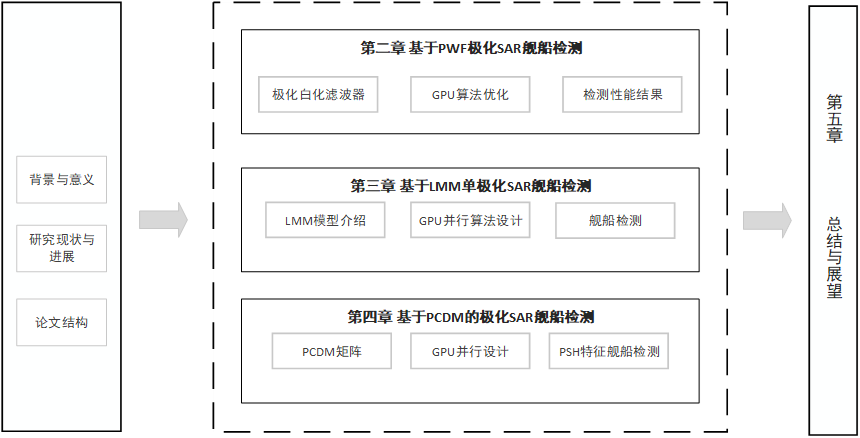
\includegraphics[width=0.85\textwidth]{structure.png}
    \caption{论文内容安排}
    \label{fig:chap1:structure}
  \end{figure}

  第二章研究基于PWF极化SAR舰船检测方法。本章首先介绍了SAR图像中斑点噪声的概念。为了抑制斑点噪声,我们将不同通道的极化信息进行融合。
  并推导出当海杂波散射矢量满足复高斯分布时的极化白化滤波器参数计算公式。之后采用极化白化滤波器生成重构图像,并应用CFAR检测器进行检测。
  本章在完成算法流程分析后,设计了基于GPU的并行极化白化滤波器舰船检测算法与多GPU协同实现的方案。最后通过实验,我们验证了基于GPU算法的有效性
  与高校性。

  第三章研究了基于混合对数正态模型的单极化SAR舰船检测方法。本章我们首先介绍了混合对数正态分布的概念与其参数
  估计方法。然后使用LMM模型对海杂波进行建模并应用CFAR检测器进行检测。针对该算法中迭代计算分布参数的过程,本章提出了
  基于GPU的优化方案,最后实验结果证明本章的基于GPU的方法在算法时间性能上获得了数十倍的提升。

  第四章研究了基于极化协方差差异矩阵的极化SAR舰船检测方法。本章我们首先回顾了极化SAR散射表征与SPAN理论,并对极化协方差差异矩阵
  做了详细的介绍。我们提取了极化协方差差异矩阵的SPAN值与PSH特征用于舰船目标检测并阐述了该算法在GPU上实现的具体细节,最后通过实验证明了本章基于GPU的
  PCDM舰船检测方法检测效果相较于PWF方法在时间性能与检测精度上都有明显的提升。

  第五章对本文的工作进行了总结并提出了对未来工作的展望。